% Chapter Template

\chapter{Analysis of microscopy images to obtain network architecture} % Main
% chapter title

\label{Chapter-Image} % Change X to a consecutive number; for referencing this
% chapter elsewhere, use \ref{ChapterX}

\lhead{Chapter 2. \emph{Analysis of microscopy images to obtain network
architecture}}
% Change X to a consecutive number; this is for the header on each page - perhaps a shortened title

%----------------------------------------------------------------------------------------
%	SECTION 1
%----------------------------------------------------------------------------------------
\section{Introduction}
The geometric structure, also called here: architecture or topology of a
biopolymer network impacts its mechanical properties and biological functions.
The goal of this chapter is to explain the algorithms and software used to
obtain the network structure from experimental measurements. To accomplish that,
first we will introduce some filters and middle-steps used in the process. Second, we will explain the two
methods that we have tested, FIRE and Avizo. At the same time, using confocal
images of actin networks obtained from our lab,  we will extract statistical
distributions of some properties of the network using both algorithms. Finally
we will compare the results from both algorithms, and comment about future
directions and improvements.

\subsection{Notation:}


 We define the \textbf{pixel} or \textbf{pixel position}, in the stack of images as:
 $\vect{p}\equiv(x,y,z)\, \epsilon \,V$, where
 $x\eps{}[1,X]$, $y\eps{}[1,Y]$, $z\eps{}[1,Z]$ are the integer coordinates and
 $V\subset \mathbb{I}^3$ is the volume of the stack of images $V=\{X\times
 Y\times Z\}$.
 With $Z$ the number of images in the stack, and $X,Y$ the size of the $2D$ images.
 
 \textbf{Pixel value} refers to the value of the pixel in the corresponding
 image.
 The value could be an Integer, a Boolean, or a Real number, depending if we are
 talking about a gray-scale image, a binarized image, a distance map,
 or anything else which has been previously defined.

 The original \textbf{gray-scale image} $I$ is defined as:
 $I(\vect{p}):V \longrightarrow G$ where
 $G$ is a set of integers representing the gray-scale.
 $G=\{0,1,\ldots,G_M\}\subset\mathbb{I}$ where $0$ represents black, $G_M$
pure white, and the others correspond to different gray-scale values. $G_M=255$
in $8$ bits images, and $G_M=2^{16} - 1 = 65535$ in higher quality images of $16$ bits. 

The \textbf{binarized image} B is defined as the map:
$$f_B: I \longrightarrow B_T \,\,|$$ 
\begin{equation}
 B_T(\vect{p})=
   \begin{cases} 
     1               & \mbox{if } I(\vect{p}) > T   \\
     0               & \mbox{if } I(\vect{p}) < T
   \end{cases}
   \label{eq:bin}
\end{equation}
Where $T\eps{}G$ is the threshold value of the binarization. The threshold can also be expressed as
a normalized intensity value $T_P \eps{}[0,1]\subset \mathbb{R}$. If 
$I_{max}\eps{}G$ is the max value of $I$, then the threshold  is
$T=round(T_P \cdot I_{max})$  where the round function converts a real number
into the nearest integer. The binary threshold can also be characterized with a percentage of the
brightest gray-scale value involving
cumulative histograms of $I$.

\section{Filters: steps of the process}
The following filters are shared, with differences, in both methods of
extraction of the spatial graph. A network or graph is defined by two sets:
a set of nodes (i.e. cross-links), characterized by their spatial position; and
by a list of edges (i.e. links), connecting pairs of those nodes.
\subsection{Image thresholding}
The gray levels of pixels belonging to an object are substantially
different from the gray levels of the background. Thresholding is a way to
separate objects from the background.

\begin{figure}[h]
\begin{center}
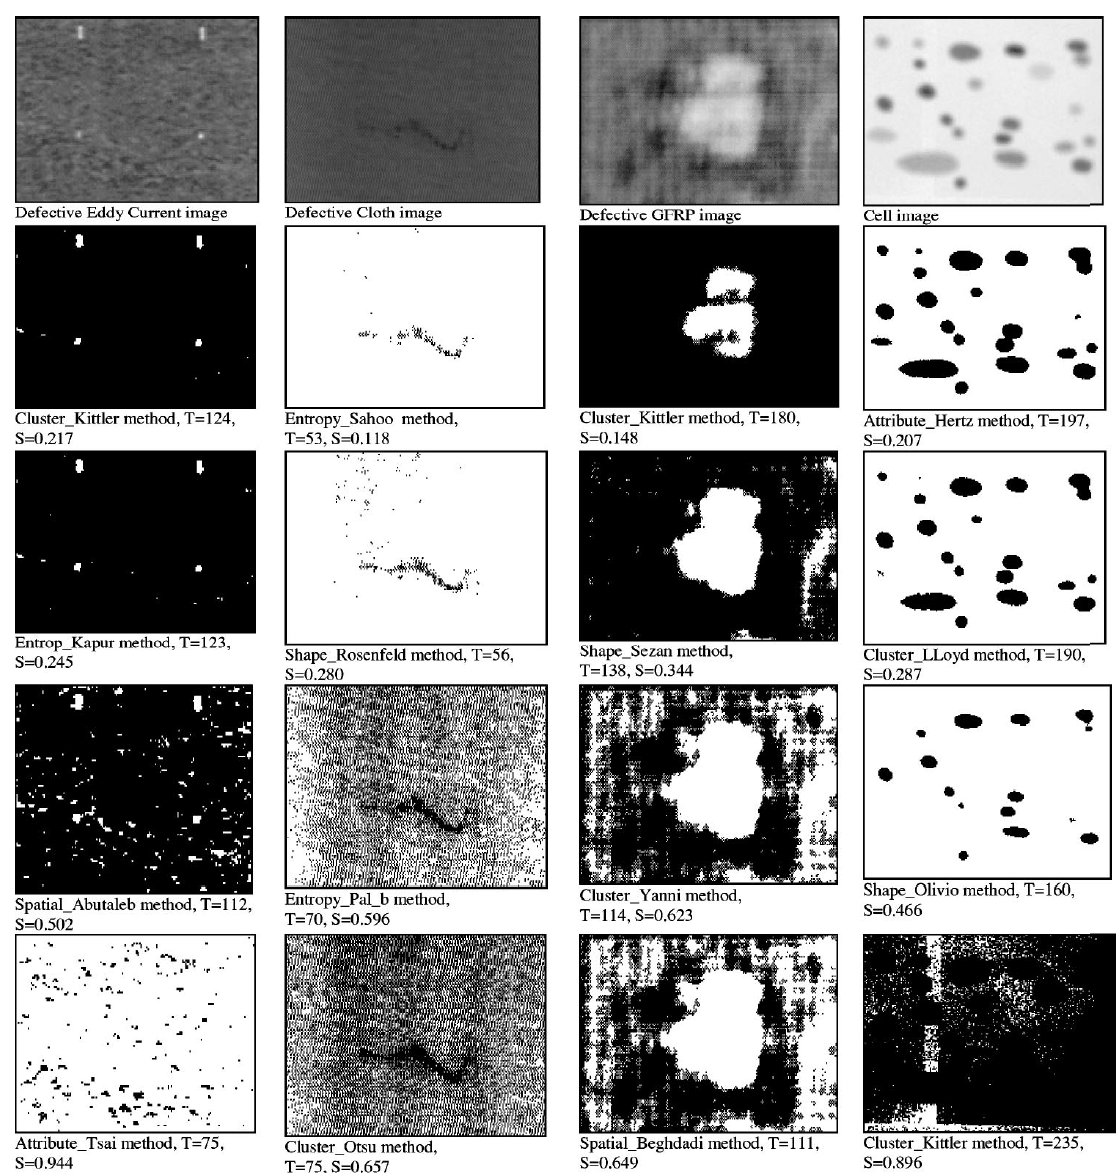
\includegraphics[width=0.9\textwidth,
height=0.6\textwidth]{Figures/chapter-image/fig_threshold_image.png}

\caption[Threshold calculation by different methods]{Different thresholding
results on sample images from Ref.\citep{sezgin_survey_2004}}
\label{fig:threshold}
\end{center}
\end{figure}

\citet{sezgin_survey_2004} is a good review about the subject. The output of the
thresholding process is a binary image, whose one state will indicate the
foreground objects, while the complementary state will correspond to the
background.\\
\begin{equation}
P'_i=
   \begin{cases} 
     1               & \mbox{if } I(\vect{p}) > T   \\
     0               & \mbox{if } I(\vect{p}) < T
   \end{cases}
   \label{eq:bin}
\end{equation}
Where $P'_i\,\epsilon \, \{0{,} 1\}$ is the binarized output pixel , $P_i\,
\epsilon \,[0{,}255]$ is the gray-scale input pixel, and $T\,
\epsilon \,[0{,}255]$ is the threshold value. Note that the max value in the
grey scale could vary depending of the number of bits of the image. $255$ is
the max value for $8$ bits images;
in the case of high quality images of $16$ bits, the max value will rise to
$2^{16} - 1 = 65535$. In both cases the max value corresponds to pure white and
$0$ to black.

\begin{figure}[h]
\begin{subfigure}{0.5\textwidth}
  \centering
  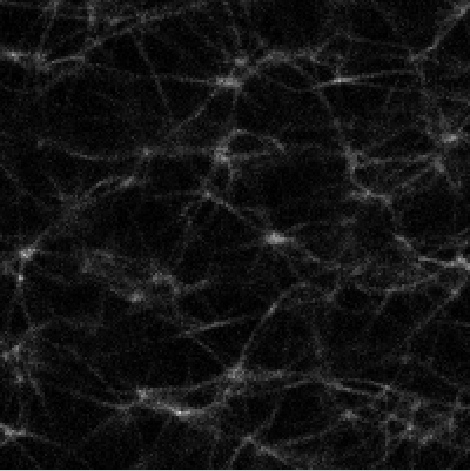
\includegraphics[width=0.9\textwidth]{Figures/chapter-image/binary/fig_bin_original.png}%
  \caption{Input Image - Original}
  \label{binoriginal}
\end{subfigure}%
\begin{minipage}{0.5\textwidth}
  \centering
  \begin{subfigure}{0.5\textwidth}
    \centering
    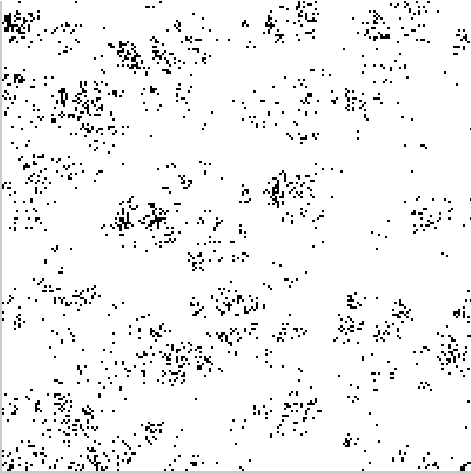
\includegraphics[width=0.9\textwidth]{Figures/chapter-image/binary/fig_bin_01.png}%
    \caption{$T_P$=0.01}
    \label{bin001}
  \end{subfigure}%
  \begin{subfigure}{0.5\textwidth}
    \centering
    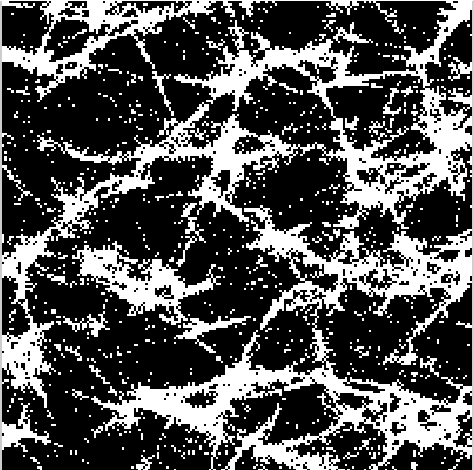
\includegraphics[width=0.9\textwidth]{Figures/chapter-image/binary/fig_bin_08.png}
    \caption{$T_P$=0.08}
    \label{bin008}
  \end{subfigure}

  \begin{subfigure}{0.5\textwidth}
    \centering
    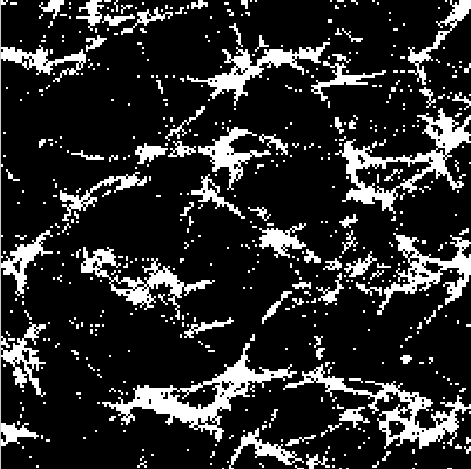
\includegraphics[width=0.9\textwidth]{Figures/chapter-image/binary/fig_bin_01176Otsu.png}%
    \caption{$T_P$=0.1176}
    \label{binotsu}
  \end{subfigure}%
  \begin{subfigure}{0.5\textwidth}
    \centering
    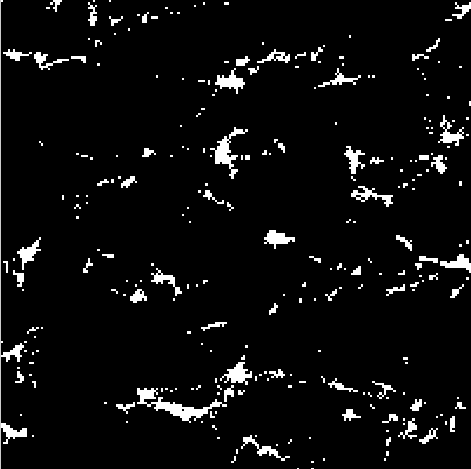
\includegraphics[width=0.9\textwidth]{Figures/chapter-image/binary/fig_bin_20.png}%
    \label{bin020}
    \caption{$T_P$=0.20}
  \end{subfigure}%
\end{minipage}

\caption[Different threshold values on networks]{Different threshold values in
Actin network.
$T_P$ is a normalized threshold value, if $G_{max}$ is the brightest pixel, then
$T=T_P\cdot P_{max}$. According to eq \ref{eq:bin}, any pixel which value is greater than T transforms to $1$
(white) after the binary filter.
At low values of threshold (case \subref{bin001}), we have blurred networks, but
at high values (case \subref{bin020}), some connectivity information is lost.
The case \subref{binotsu} corresponds to the threshold calculated by the Otsu's
method } 
\label{fig:binary}
\end{figure}

There is a lot of research in thresholding. One of the most famous binary
filters is Otsu's method, which is usually implemented by default in commercial software.
Otsu's method minimizes the weighted sum of within-class variances of the
foreground and background pixels to establish an optimum threshold
\citep{sezgin_survey_2004}. This method belongs to the clustering-based methods
of thresholding. Further classification of thresholding is based on:
\begin{itemize}
  \item \textbf{Histogram shape.} Peaks, valleys and curvatures of the smoothed
  gray-level histogram are analyzed. \emph{Peak-and-valley}
  \item \textbf{Clustering.} The gray levels are clustered in two parts, one
  corresponding to the background and the other to the foreground. This method
  analyses separately each cluster. \emph{Otsu, Minimum error, fuzzy}.
  \item \textbf{Entropy.} Exploits the entropy of the distribution of the gray
  levels in the image. Maximization of entropy is indicative of high information transfer.
  Low cross-entropy between input gray level and output binary means
  preservation of information. \citet{pal_automatic_1983}
  were the first to use Shannon entropy in image analysis.
 \citep{pal_image_1988}
  \item \textbf{Object attribute.} Select the threshold based on some attribute
  quality between the original and binarized image. \emph{Edge matching, connectivity,
  shape compactness}.
  \item \textbf{Spatial methods}. This class not only uses the gray
  distribution, also studies the dependency of pixels in a neighborhood, for example, correlation
functions or co-ocurrence probabilities.
  \item \textbf{Local adaptive methods.} A threshold is calculated at each
  pixel, which depend on some local statistics, like \emph{variance}.
\end{itemize}



For our purposes, the binarization threshold will have an impact obtaining the
network. If the threshold is too high, long fibers will break in short,
unconnected pieces. If the threshold is too low, fibers that are clearly
separated, will become blurred together.

In Fig.\ref{fig:binary}
we compare the geometry of a small area of an actin network after
applying different binary thresholds. The stack of images of
networks used here was obtained in our group by Dr. Allan
Raudsepp using confocal microscopy on actin.
 


\subsection{Distance maps}

The distance map calculates the distance from a
white pixel to the nearest black pixel. Every white pixel in the binary image
has now a real value calculated using any selected distance function (euclidean,
quasi-euclidean,\ldots ). Distance maps can be applied to a binary image, or to
any image with shapes that are labeled differently.
Fig.\ref{fig:distancemap} has some distance maps of actin networks.
We can see in Fig.\ref{fig:fire_LMPS} the values of a distance map, which have
been simplified from real to integers for clarity.
 
 
\begin{figure}[h]
\begin{minipage}{0.5\textwidth}
  \centering
  \center{\textbf{Binarization}}\\
  % \begin{minipage}{0.5\textwidth}
  \begin{subfigure}{0.5\textwidth}
    \centering
    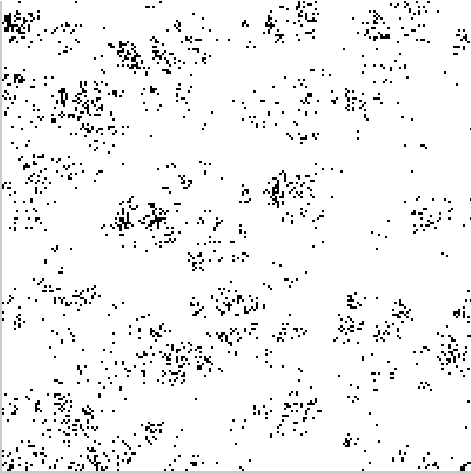
\includegraphics[width=0.9\textwidth]{Figures/chapter-image/binary/fig_bin_01.png}
    \caption{$T_P$=0.01}
  \end{subfigure}%
  \begin{subfigure}{0.5\textwidth}
    \centering
    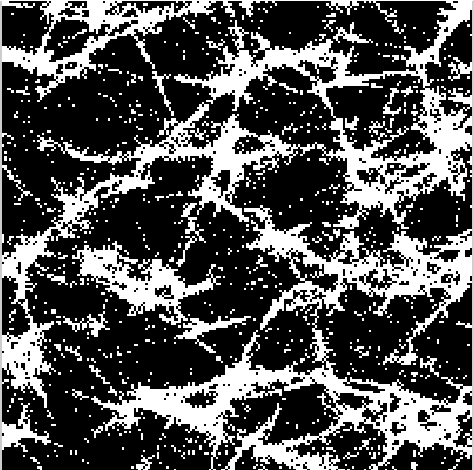
\includegraphics[width=0.9\textwidth]{Figures/chapter-image/binary/fig_bin_08.png}
    \caption{$T_P$=0.08}
  \end{subfigure}

  \begin{subfigure}{0.5\textwidth}
    \centering
    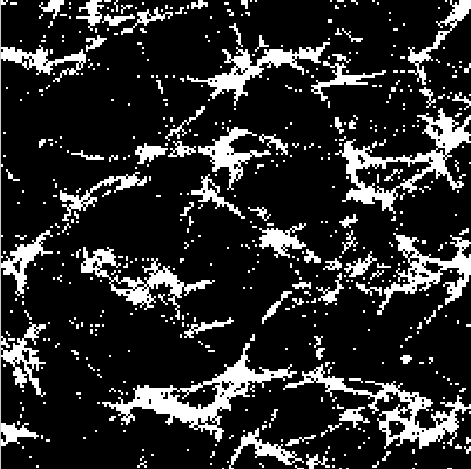
\includegraphics[width=0.9\textwidth]{Figures/chapter-image/binary/fig_bin_01176Otsu.png}
    \caption{0.1176}
  \end{subfigure}%
  % \hspace{1pt}
  \begin{subfigure}{0.5\textwidth}
    \centering
    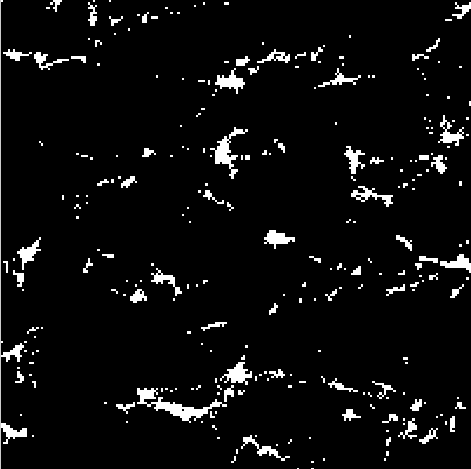
\includegraphics[width=0.9\textwidth]{Figures/chapter-image/binary/fig_bin_20.png}
    \caption{$T_P$=0.20}
  \end{subfigure}%
\end{minipage}
\begin{minipage}{0.5\textwidth}
  \centering
  \center{\textbf{Distance map}}\\
  \begin{subfigure}{0.5\textwidth}
    \centering
    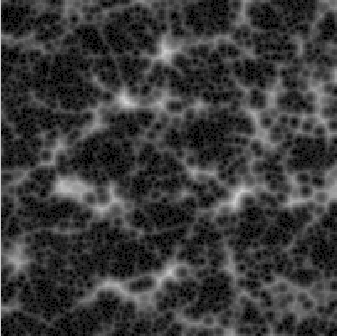
\includegraphics[width=0.9\textwidth]{Figures/chapter-image/distance/fig_dist_01.png}
    \caption{$T_P$=0.01}
  \end{subfigure}%
  \begin{subfigure}{0.5\textwidth}
    \centering
    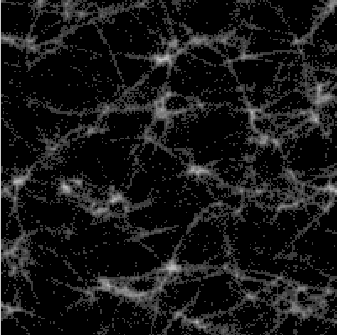
\includegraphics[width=0.9\textwidth]{Figures/chapter-image/distance/fig_dist_08.png}
    \caption{$T_P$=0.08}
  \end{subfigure}

  \begin{subfigure}{0.5\textwidth}
    \centering
    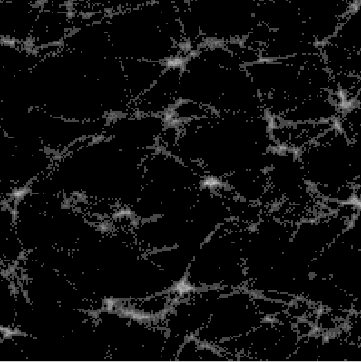
\includegraphics[width=0.9\textwidth]{Figures/chapter-image/distance/fig_dist_01176Otsu.png}
    \caption{0.1176}
    \label{distotsu}
  \end{subfigure}%
  \begin{subfigure}{0.5\textwidth}
    \centering
    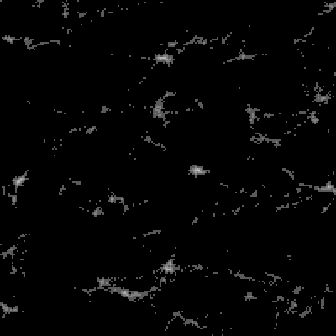
\includegraphics[width=0.9\textwidth]{Figures/chapter-image/distance/fig_dist_20.png}
    \caption{$T_P$=0.20}
    \label{dist014}
  \end{subfigure}
\end{minipage}

\caption[Distance map - Actin]{ Distance maps calculated from binarized images
with different normalized thresholds $T_P$}
\label{fig:distancemap}
\end{figure}
 
\subsection{Skeletonization}
The skeleton of an object is a representation of the object, which contain both,
shape features and topological structures of the original object. It is widely
used in computer graphics, character recognition, and analysis of biomedical
images.\citep{bai_skeleton_2007,golland_fixed_2000,ge_generation_1996}. The
skeletonization is very sensitive to noise and boundary deformations, which generates redundant skeleton branches that disturb the
topology of the skeleton graph (Fig.\ref{fig:skeleton-fixedtopo}(b)).

To overcome this instability, the methods used are based on skeleton pruning,
i.e. eliminating the spurious branches. What are then the desirable properties
of a skeletonization process?
\begin{enumerate*}[label=\textbf{\alph*)}]
  \item Preserve the topology of the original object, i.e. it has the same tails
  and/or holes.
  \item Accurate position.
  \item Contain the centers of maximal disks, which can be used for the
  reconstruction of the original object
  \item Stable under small deformation and noise. 
  
\end{enumerate*}

The most important skeletonization algorithms
can broadly be classified into two types:

\begin{enumerate}

  \item Based on Voronoi diagrams \citep{ogniewicz_hierarchic_1995}. 
These methods search the locus of centers of the maximal disks
contained in the contour of the object. The skeleton can be
extracted with accurate position and topology, but the time
of computation is usually prohibitive, and the complicated skeleton needs to be
pruned.
  \item Based on detecting ridges
  in the distance map from the boundary points. The
  position is accurate, but does not guarantee correct topology
  \citep{ge_generation_1996}. It is widely used because the computation
  affordability. The two methods used here to analyse the networks are based on
  this kind of skeletonization. 
\end{enumerate}
 

\begin{figure}[h]
\begin{center}
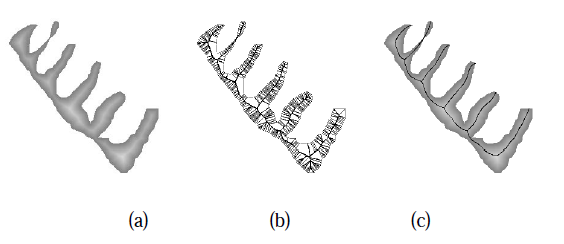
\includegraphics[width=0.8\textwidth]{Figures/chapter-image/skeleton-fixedtopo_letters.png}%
\caption[Skeletonization]{Skeletonization process. (a) Distance
map. (b) Traditional skeleton with no pruning. (c) Skeleton generated using
fixed topology methods. From Ref.\citep{bai_skeleton_2007,golland_fixed_2000}}
\label{fig:skeleton-fixedtopo} 
\end{center}
\end{figure}
 
 
 
 
\section{FIbeR Extraction -FIRE-}

FIRE has been developed by Andrew M.Stein
  \citep{stein_mathematical_2007} to extract collagen networks from confocal
  images. It can be downloaded, and upgrades can be uplodaded in
  \url{https://github.com/uw-loci/fiber-extraction}. The method
  \citep{stein_algorithm_2008} is based on an original idea of
  \citet{wu_automated_2003}. The main upgrade is the use of multiple nucleation
  points   and the restriction that each branch extends only  in a single 
  direction from a nucleation point. In \citet{wu_automated_2003}  the network has a single nucleation point at the global maximum of the distance function D.


 \begin{enumerate}[label=\textbf{\Alph*}]
 
 \item \textbf{Smooth filter} Smooth the image with a Gaussian filter
 \item \textbf{Binarization threshold} Keep a percentage of the brightest pixels
 \item \textbf{Distance map D} Distance map using Euclidean distance. It
 assigns a value to each pixel equal to the distance from that pixel to the nearest black value.

 \item \textbf{Nucleation points NPs} They are the
 local maxima of the distance map $D(\vect{u})$. The locality is defined by a
 box of chosen radius $s_{xbox}=5$. They are only selected if they
 exceeds a tunable threshold $\theta_{nuc}=2$. A single nucleation point of
 value $4$ is denoted by the thick circle in \ref{fig:fire_LMPS}\subref{LMP1}
 
 \item \textbf{Extension of branches LMPs} The next step is to trace the
 branches, extending from the nucleation points. To do that FIBER finds a set of
 Local Maximum Points (LMPs) at \emph{each} nucleation point. LMPs occur where
 there is a local maximum in $D(\vect{u})$ on the surface of the box centered in the NP
 $\vect{u}$, and with radius(in pixels) the rounded up value of $D(\vect{u})$.
 See Fig. \ref{fig:fire_LMPS}\subref{LMP1}. LMPs are then extended with other
 LMPs only if the direction of extension is straight enough
 (Fig. \ref{fig:fire_LMPS}\subref{LMP2}). If there is no LMP with that
 condition, or it arrives other nucleation point, the iteration ends.
 \end{enumerate}


\begin{figure}[h]
  \centering
  \begin{subfigure}{0.5\textwidth}
    \centering
    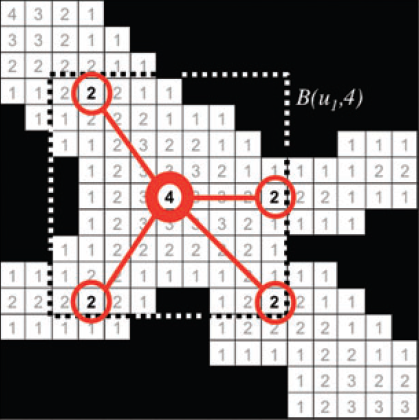
\includegraphics[width=0.8\textwidth]{Figures/chapter-image/fire/nucleation1.png}%
    \caption{Step 1}
    \label{LMP1}
  \end{subfigure}%
  \begin{subfigure}{0.5\textwidth}
    \centering
    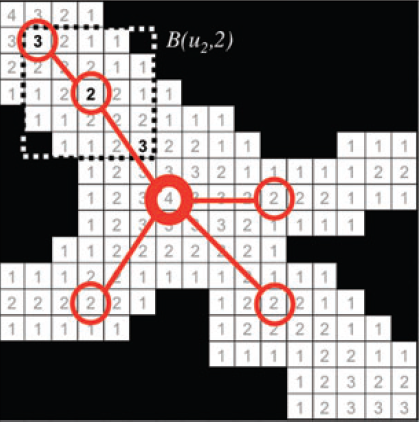
\includegraphics[width=0.8\textwidth]{Figures/chapter-image/fire/nucleation2.png}
    \caption{Step 2}
    \label{LMP2}
  \end{subfigure}
  \caption[FIRE algorithm - Find LMP]{Tracing of the ridges of the distance
    map using FIRE from Ref.\citep{stein_algorithm_2008}: \subref{LMP1} Step 1:
    Pick a nucleation point (thick circle) and find all LMPs. \subref{LMP2} Step 2:
    Pick an LMP and find the next LMP which continues in the same direction. See
  text for details.}
  \label{fig:fire_LMPS}
\end{figure}





 
 
\subsection{Results in FIRE}
 I have used FIRE to analyse our
 confocal stacks obtained from actin networks. For testing purposes, the images
have been cropped due to the slowness of FIRE
processing big networks. From an original image of Actin of
$V=1024\times1024\times39$, we have cropped it to $V=200\times200\times20$. 

In Fig.\ref{fig:fire_stepbystep} we can see the different steps of the FIRE
algorithm. In Fig.\ref{fig:fire_histograms} we plot the statistical distribution
of length and degree for different thresholds $T_P$. Further analysis is
required, and a bigger network for better statistics, but it seems that length
follow a log-normal distribution, and the degree, a geometrical distribution. We
will say more about distributions in chapter \ref{Chapter-Reconstruction}.

 \begin{figure}[h]

\begin{center}
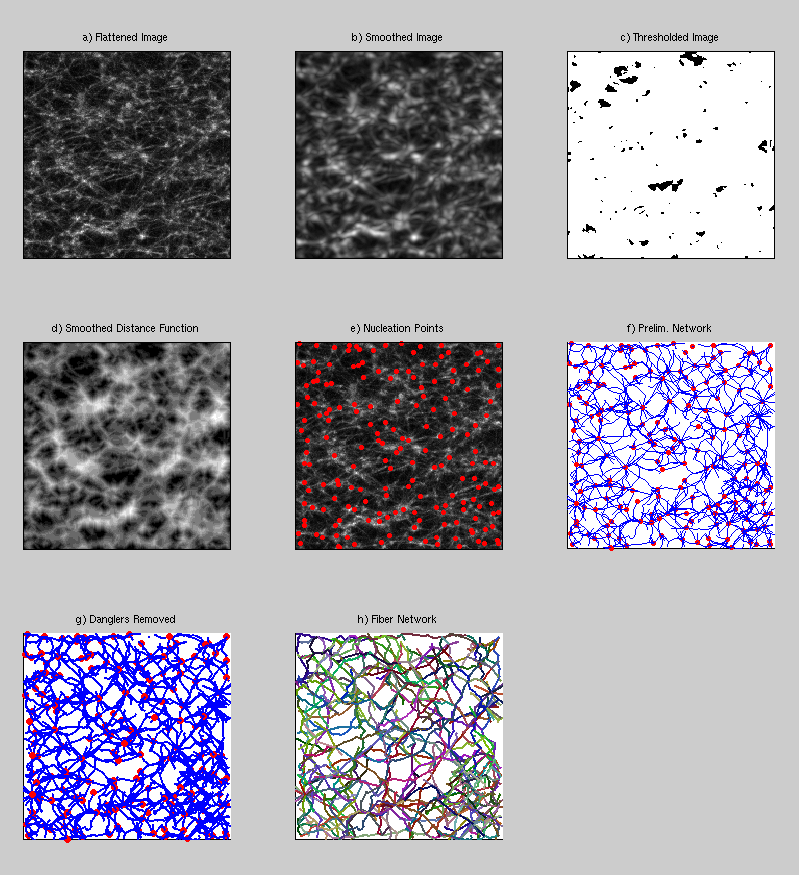
\includegraphics[width=0.9\textwidth]{Figures/chapter-image/fire/fire012.png}%

\end{center}


\caption[Fire: Step by step for $T_P=0.12$]{FIRE: step by step}
\label{fig:fire_stepbystep}
\end{figure}

\begin{figure}[h]
  \centering
  \begin{subfigure}{0.5\textwidth}
    \centering
    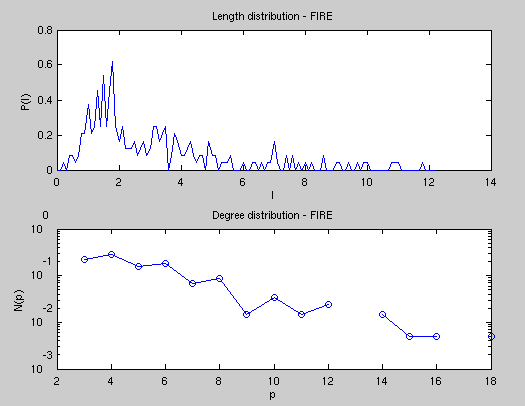
\includegraphics[width=0.95\textwidth]{Figures/chapter-image/fire/fire017histo.png}%
    \caption{$T_P=0.17$}
    \label{firehisto017}
  \end{subfigure}%
  \begin{subfigure}{0.5\textwidth}
    \centering
    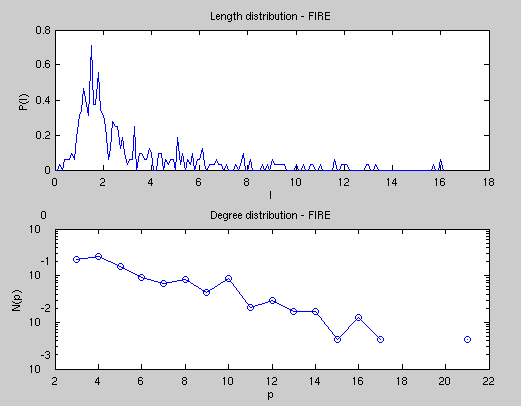
\includegraphics[width=0.95\textwidth]{Figures/chapter-image/fire/fire012histo.png}%
    \caption{$T_P=0.12$}
    \label{firehisto012}
  \end{subfigure}

  \begin{subfigure}{0.5\textwidth}
    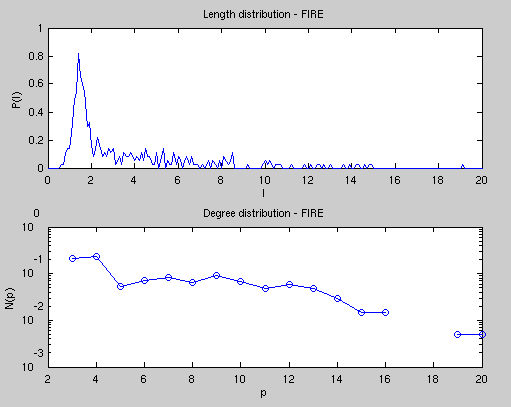
\includegraphics[width=0.95\textwidth]{Figures/chapter-image/fire/fire008histo.png}%
    \caption{$T_P=0.08$}
    \label{firehisto008}
  \end{subfigure}
\caption[Distributions of length and degree in FIRE]{Extracting statistical
distributions for different binary thresholds using FIRE from cropped
actin netwoks.}
\label{fig:fire_histograms}
\end{figure}

An useful statistical distribution is the one studying the angles between edges
that are incident to the same node. I am currently working on a way to extract
the director cosines (angles) distribution from FIRE.

\section{Avizo: XSkeleton}
 Avizo is a software commercialized by
 \href{http://www.vsg3d.com/avizo/overview}{FEI: Visualization Sciences Group}.
The access to Avizo is granted by a collaboration with Fonterra (Food company,
NZ).

\textbf{XSkeleton} is the package or module that we will use to extract the
network topology. The algorithm and the result is different to FIRE. Here
follows a description step by step:
\begin{enumerate}[label=\textbf{\Alph*}]
 \item\textbf{Smooth filter} Smooth the image with a Gaussian filter
 \item\textbf{Binarization threshold} Multi-threshold module. This threshold is
 not based in percentage of the brightest pixel. It is a classical threshold turning
 to pure white $255$ or logical $1$ all pixels with a value greatest than the
 threshold value, and black $0$ all the pixels below that value.
 \item\textbf{Distance map} Distance map using Euclidean distance. It assigns a
 value to each pixel equal to the distance from that pixel to the nearest black value. 
 \item\textbf{Thinner module} This is the \textbf{skeletonization} step. The
 module takes as input a label-field to be thinned and a distance map scalar field. It removes voxel by voxel from the segmented
 object until only a string of connected voxels remains.
 The thinning algorithm automatically detects dead end branches of skeleton
 spatial graphs. A parameter is used to distinguish them from noise on the
 interface  of the considered regions to avoid spurious branches.  Its default
 value is 5, i.e. the branches with a dead end which length is lower  than 5
 voxels are automatically considered as noise and removed.  Setting this to 10,
 which is a rather large value, leads to only a few branches remaining in the
 skeleton.  The drawback is that you also might miss real endpoints.
 
\item\textbf{Trace lines module} Converts an image that contains lines
represented by voxels into a spatial graph object.

 \end{enumerate}

\begin{figure}[h]

% \begin{minipage}{0.5\textwidth}
 
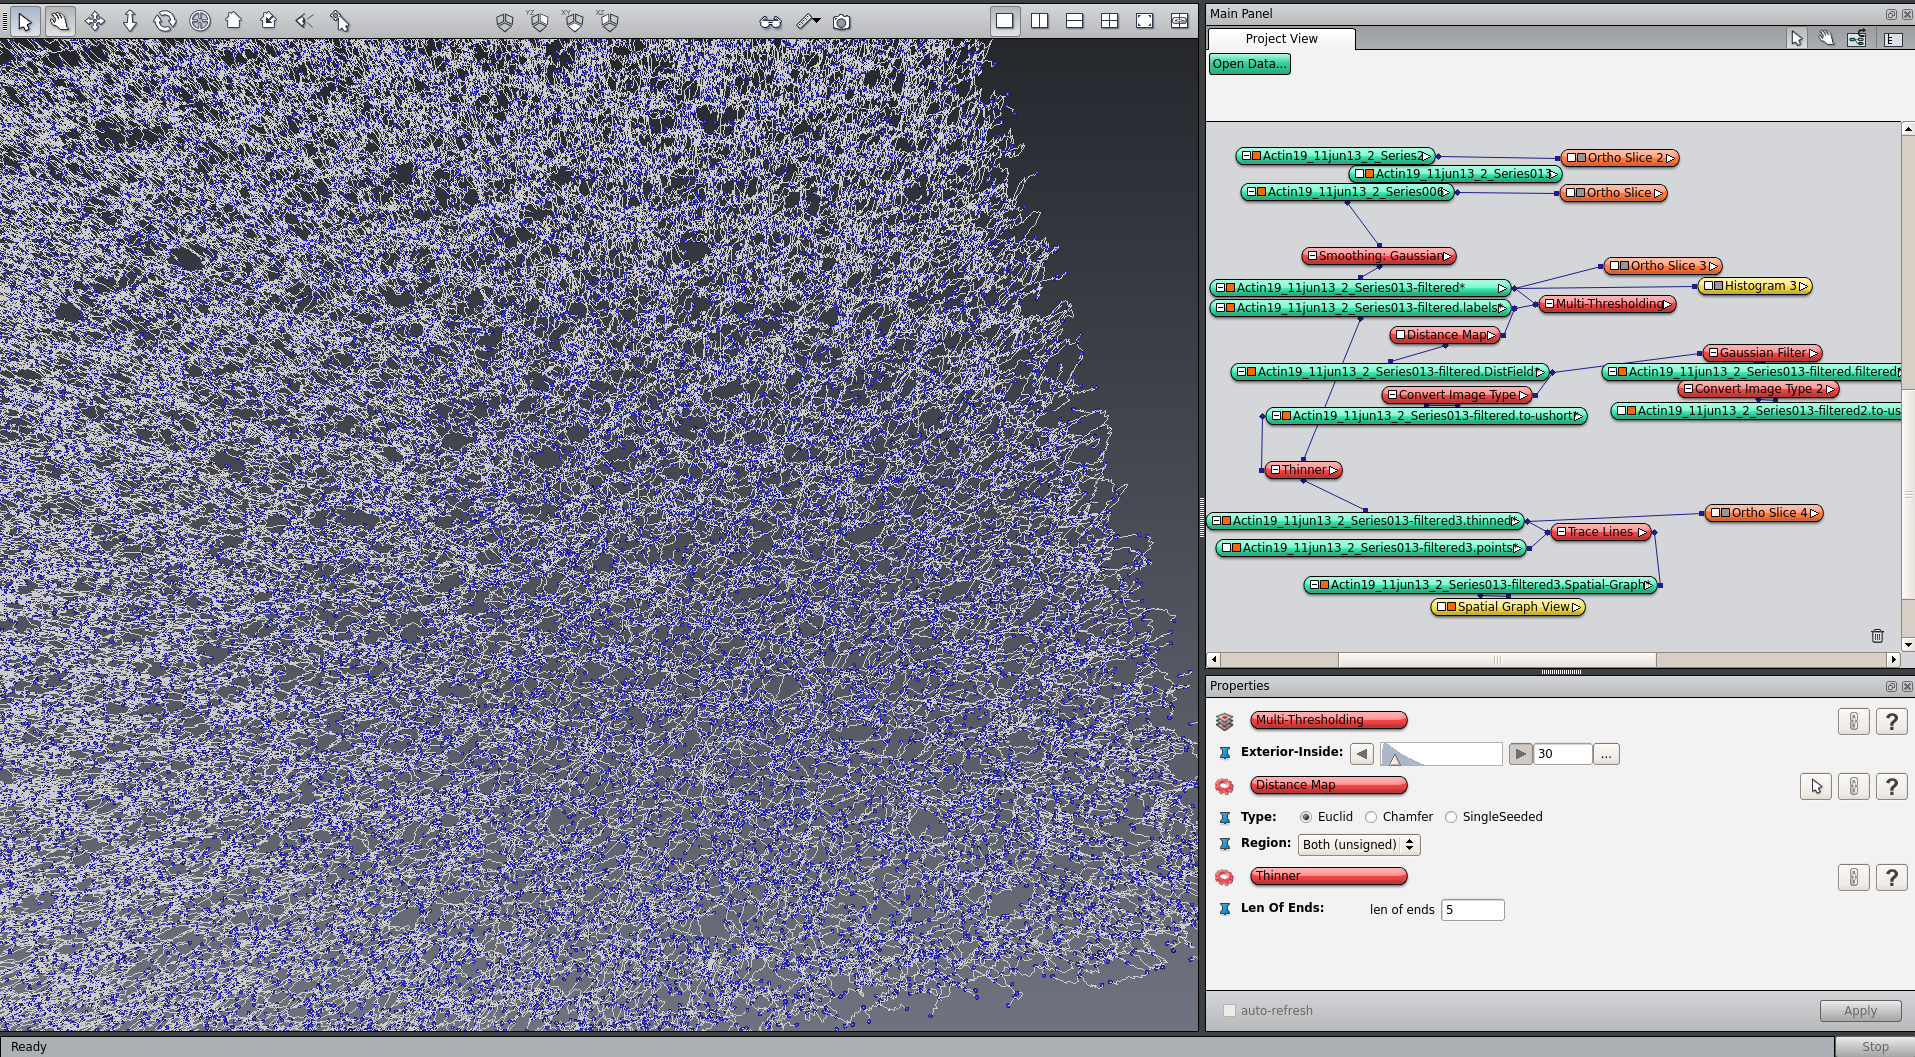
\includegraphics[width=0.9\textwidth]{Figures/chapter-image/avizo/workspace-wholedata.png}%

\caption[Avizo image: Actin network visualization and workspace]{Avizo
workspace. \emph{Left:} Visualization of the whole network of Actin data.
\emph{Top right:} Filters applied step by step. \emph{Bottom right:} Most
influential filters parameters, binarization threshold ($30$ in the image) and
skeletonization parameter: pruning of branches that length is lesser than the
threshold ($5$ in the image)}
\label{fig:avizo_workspace}
\end{figure}


\subsection{Avizo results:}
We have analyzed the whole stack of our confocal images of actin
($V=1024\times1024\times39$). The key parameters in Avizo are the binarization
$T$ and the pruning threshold $P$.

In Fig.\ref{fig:avizo_workspace}, a regular workspace in Avizo can be seen. The
different filters, the key parameters, and the result of the process, the actin
network are visualized.

In Fig.\ref{fig:avizo_histograms30} we have extracted statistical distributions
from the network that will be used in chapter \ref{Chapter-Reconstruction} for
the reconstruction of the network. 

In Fig.\ref{fig:avizo_histograms21} we can check that statistical distributions
are quite robust versus small changes in the key parameters $T$ and $P$.

\begin{figure}[h!]
  \centering
  \begin{subfigure}{0.32\textwidth}
    \centering
    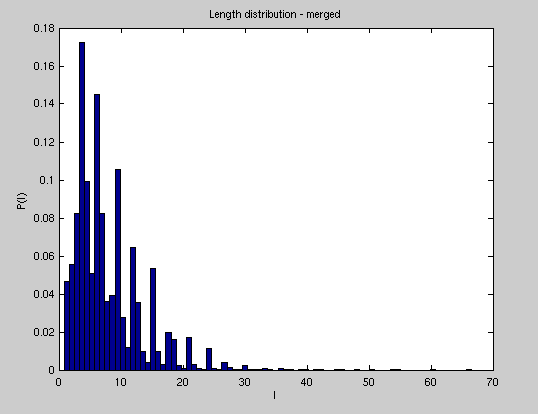
\includegraphics[width=0.92\textwidth]{Figures/chapter-image/avizo/ActinZ39b21l5-histo-length.png}%
    \label{avizo305-length}
  \end{subfigure}%
  \begin{subfigure}{0.32\textwidth}
    \centering
    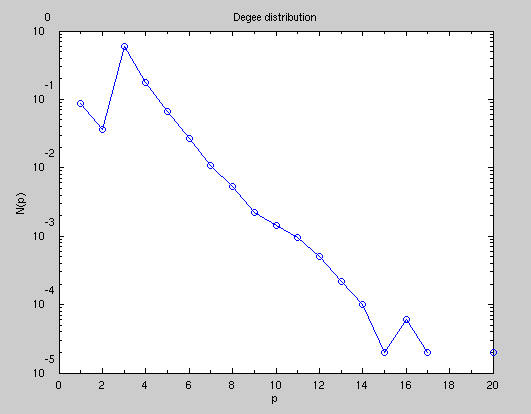
\includegraphics[width=0.92\textwidth]{Figures/chapter-image/avizo/ActinZ39b21l5-histo-degree.png}%
    \label{avizo305-degree}
  \end{subfigure}%
  \begin{subfigure}{0.32\textwidth}
    \centering
    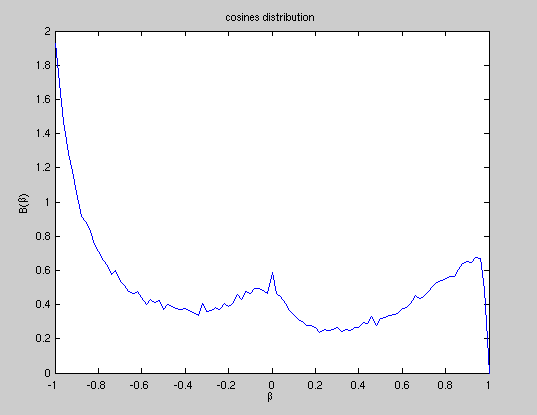
\includegraphics[width=0.92\textwidth]{Figures/chapter-image/avizo/ActinZ39b21l5-histo-cosines.png}
    \label{avizo305-cosines}
  \end{subfigure}

  \caption[Distributions of length, degree, and cosines with Avizo for
  actin with T=30,P=5]{Actin data analyzed with Avizo with binary threshold
    $T=30$ and pruning parameter $P=5$. \subref{avizo305-length} Length following a
    log-normal or exponential distribution. \subref{avizo305-degree} Degree
    following a geometrical distribution. \subref{avizo305-cosines}  Director
  cosines following an unknown distribution}
  \label{fig:avizo_histograms30}
\end{figure}

\begin{figure}[h!]
  \centering
  \begin{minipage}{0.32\textwidth}
    \centering
    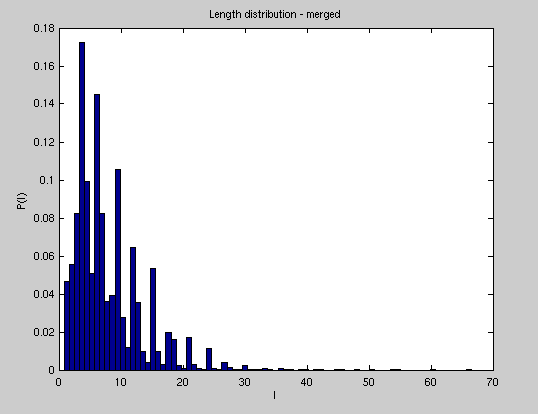
\includegraphics[width=0.92\textwidth]{Figures/chapter-image/avizo/ActinZ39b21l5-histo-length.png}%
  \end{minipage}
  \begin{minipage}{0.32\textwidth}
    \centering
    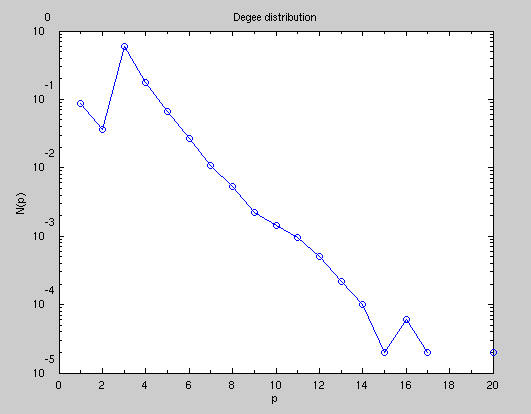
\includegraphics[width=0.92\textwidth]{Figures/chapter-image/avizo/ActinZ39b21l5-histo-degree.png}%
  \end{minipage}
  \begin{minipage}{0.32\textwidth}
    \centering
    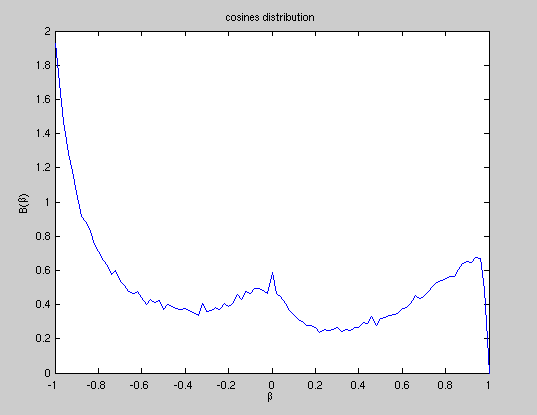
\includegraphics[width=0.92\textwidth]{Figures/chapter-image/avizo/ActinZ39b21l5-histo-cosines.png}%
  \end{minipage}
  \begin{minipage}{0.32\textwidth}
    \centering
    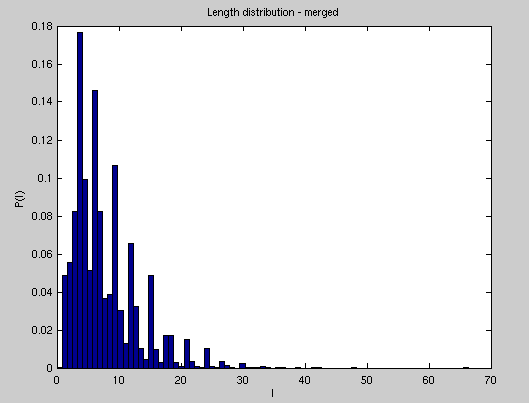
\includegraphics[width=0.92\textwidth]{Figures/chapter-image/avizo/ActinZ39b21l8-histo-length.png}%
  \end{minipage}
  \begin{minipage}{0.32\textwidth}
    \centering
    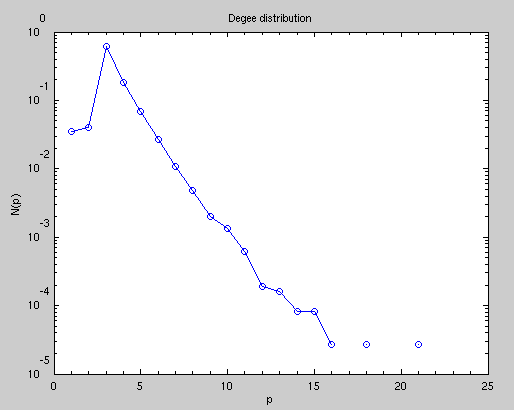
\includegraphics[width=0.92\textwidth]{Figures/chapter-image/avizo/ActinZ39b21l8-histo-degree.png}%
  \end{minipage}
  \begin{minipage}{0.32\textwidth}
    \centering
    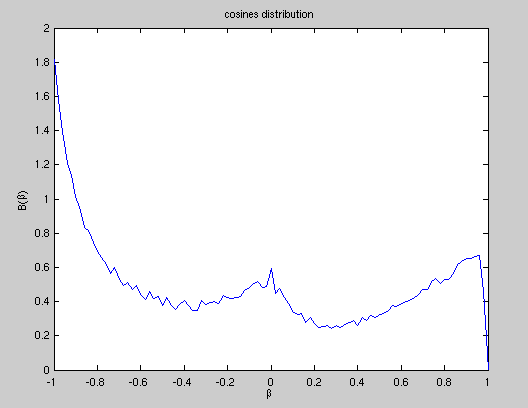
\includegraphics[width=0.92\textwidth]{Figures/chapter-image/avizo/ActinZ39b21l8-histo-cosines.png}%
  \end{minipage}

\caption[Distributions of length, degree, and cosines with Avizo for
actin with T=21,P=5]{Actin data analyzed with Avizo with binary threshold
$T=21$ and pruning parameter: $P=5$ in the first row, and  $P=8$ in the second
row. We can see that small changes in the parameters
does not affect much to the statistical distributions}
\label{fig:avizo_histograms21}
\end{figure}

The statistical distribution must be further compared with those in FIRE (with
a whole network), but we can see that the algorithm seems stable against minor
changes in the important parameters.

\section{Conclusions}
The comparison between the FIRE algorithm in Matlab and Avizo is not trivial.
Here I select the most important:

{\large\textbf{FIRE algorithm in Matlab}}
\begin{itemize}
\item \textbf{Pros:}

\begin{itemize}
  \item \textbf{Open source code.} With the free access to the code I have the
  opportunity to change and manipulate all the process in function of my needs.
  This process is also quite instructive. 

  \item \textbf{Reliable.} This method has been tested carefully
\citep{stein_mathematical_2007}, and its reliability has been demonstrated in fluorescence confocal
images of stiff collagen filaments.
\end{itemize}
\item  \textbf{Contras:}
\begin{itemize}
  \item \textbf{No beautiful visualization.} I can implement a code to visualize
  the network in $3D$, but it is not as detailed as in Avizo
  \item \textbf{Slow.} It is not implemented using parallel capabilities, and
  can be quite slow for large networks.
\end{itemize}
\end{itemize}

{\large\textbf{Avizo}}
\begin{itemize}
  \item \textbf{Pros:}


\begin{itemize}
  \item \textbf{$3D$ filters.} All the filters, and image manipulation
  algorithms comes from the computer vision community and they work in $2D$.
  There are reliable open source libraries(tested code) of $2D$ filters, but
  not in $3D$.
  The implementation of a $3D$ from a $2D$ isn't usually that hard, but it is
  extra work that Avizo solves for you, with the drawback of having no access to
  those libraries because its condition of commercial software.
   \item \textbf{Visualization of the network.} It uses a computer graphics
   library called VTK (open source) to visualize the network in a beautiful and
   effective way.
   \item \textbf{Skeletonization.} It uses a skeletonization method based on the
   distance map that seems fast and effective. But knowing the exact algorithm
   would be helpful.
\end{itemize}
\item \textbf{Contras:}
\begin{itemize}
  \item \textbf{Commercial Software.} It is really expensive, we have access to
  it thanks to a collaboration agreement with Fonterra researchers. 
  \item \textbf{Black Box.} It
  shares the drawbacks of commercial software: it is impossible to
  manipulate it at your will to fit your requirements. Having no access to the
  algorithms is like using a black box, you don't know exactly what is
  happening behind the curtains. 
  \item \textbf{Development Toolbox.} There is a development add-on (extra
  cost), where you can create new filters and interact with the rest of the framework
  in Avizo. I have to carefully study if the efforts of learning this tool will
  have a decisive improvement in the image analysis.
\end{itemize}
\end{itemize}
FIBER algorithm seems very reliable, but I think it has
room for at least, technical improvement, such as parallel implementation.
The way it expands nucleation points using traces along the maximal ridges
of the distance map doesn't seem to be based in any well
established/optimized skeletonization algorithm from the computer vision
community. The free access to the code allow us to improve it or change it at our will.

The main drawback of Avizo is that I cannot access or alter the
skeletonization algorithm.
To solve that, I should implement my own skeletonization algorithm, using the
latest computer vision techniques\citep{bai_skeleton_2007}, and then interact with Avizo to represent the network.
The TEM microscopy analysis
requirements will be the key input to decide the way to follow.

Despite the algorithm used, we have to choose the set of parameters that best reproduces the topology (i.e.
architecture) of the network at the end of the image analysis process.
I cite \citet{stein_algorithm_2008}: ``We have found that with confocal
images of fluorescently labeled collagen, it is relatively straight forward
to chose a threshold that qualitatively appears to maintain
network topology". I agree with that affirmation but if it holds with
other materials, or other microscopy techniques (TEM) have to be tested. The
unique way to test it is to rely in the best image analyser that we have available, our brain.

To generate a network filtered by the brain, we follow the chains, count
the nodes, and draw a small volume of the network, using as unique analyzer our vision, and then
compare it with the topology of the automatized algorithm
\citep{chandran_affine_2006}.
Despite the suggested complexity of the process,
it is straight forward to choose, at least, a short range of threshold values that approximates the architecture. The
 information extracted from the image analysis process seems to be quite robust
against the fine tuning of the parameters, sharing the same shape with the
changes.
These distributions, especially the angle, differ along
different materials, as shown in the literature
\citep{lindstrom_finite-strain_2013}, and also comparing actin data from our lab
with collagen data from the literature\citep{lindstrom_biopolymer_2010}. These
differences create a good opportunity to relate them with mechanical properties of the bulk
system, in the context of non-affine networks.





